\ifx\XeTeXversion\undefined\pdfoutput=1\fi % arXiv: pdflatex; local builds with tectonic (XeTeX) skip it
\documentclass[10pt,a4paper]{article}
\usepackage[T1]{fontenc}
\usepackage[utf8]{inputenc}
\usepackage{lmodern}
\usepackage[margin=2.2cm]{geometry}
\usepackage{amsmath,amssymb}
\usepackage{booktabs,multirow,longtable,array,tabularx}
\usepackage{graphicx}
\usepackage[table]{xcolor}
\usepackage{microtype}
\usepackage{caption}
\usepackage[hidelinks]{hyperref}
\usepackage{xspace}
\usepackage[section]{placeins}
\renewcommand{\topfraction}{0.9}\renewcommand{\bottomfraction}{0.8}\renewcommand{\textfraction}{0.07}\renewcommand{\floatpagefraction}{0.8}\setcounter{totalnumber}{6}\setcounter{topnumber}{4}

% ---------------------------------------------------------------- numbers
% Every number in the prose comes from numbers.tex (generated by mktex.py from the analysis JSON);
% \nm{key} prints it, and a missing key prints a visible marker instead of a silent gap.
\newcommand{\defnum}[2]{\expandafter\def\csname num@#1\endcsname{#2}}
\newcommand{\nm}[1]{\ifcsname num@#1\endcsname\csname num@#1\endcsname\else\textbf{\textcolor{red}{??#1??}}\fi}
% generated by mktex.py from J-all.json; do not edit
\defnum{A-gm}{3.0}
\defnum{A-lowq}{64}
\defnum{A-lowq-graph}{19}
\defnum{A-lowq-part}{45}
\defnum{A-max}{6.4}
\defnum{A-min}{1.5}
\defnum{A-n}{34}
\defnum{A-oursbest}{34}
\defnum{A-records}{12,525}
\defnum{B-records}{3,343}
\defnum{R-amd}{10}
\defnum{R-arm}{6}
\defnum{R-box}{10}
\defnum{R-intel}{5}
\defnum{R-mac}{4}
\defnum{build-ours-h}{5.6}
\defnum{build-ours-peak}{15.7}
\defnum{build-ours-s}{20,303}
\defnum{build-rival-max-cores}{109,506}
\defnum{build-rival-max-s}{6,844}
\defnum{cold-ours-amd}{3.1}
\defnum{cold-ours-arm}{3.4}
\defnum{cold-ours-intel}{3.5}
\defnum{cold-rivalmax-amd}{19.1}
\defnum{cold-rivalmax-arm}{19.8}
\defnum{cold-rivalmax-intel}{23.8}
\defnum{cold-rivalmin-amd}{3.9}
\defnum{cold-rivalmin-arm}{4.0}
\defnum{cold-rivalmin-intel}{4.1}
\defnum{delta}{0.005}
\defnum{faster-large}{13}
\defnum{faster-mid}{11}
\defnum{faster-small}{14}
\defnum{gm-all-098}{0.96}
\defnum{gm-all-099}{1.22}
\defnum{gm-all-0995}{1.23}
\defnum{gm-amd-098}{1.02}
\defnum{gm-amd-099}{1.25}
\defnum{gm-amd-0995}{1.39}
\defnum{gm-arm-098}{0.96}
\defnum{gm-arm-099}{1.14}
\defnum{gm-arm-0995}{1.08}
\defnum{gm-box-098}{0.85}
\defnum{gm-box-099}{1.09}
\defnum{gm-box-0995}{1.09}
\defnum{gm-intel-098}{0.87}
\defnum{gm-intel-099}{1.16}
\defnum{gm-intel-0995}{1.21}
\defnum{gm-large}{1.99}
\defnum{gm-mac-098}{1.25}
\defnum{gm-mac-099}{1.69}
\defnum{gm-mac-0995}{1.56}
\defnum{gm-mid}{1.20}
\defnum{gm-small}{0.90}
\defnum{gmn-all-098}{76}
\defnum{gmn-all-099}{73}
\defnum{gmn-all-0995}{52}
\defnum{gmn-amd-098}{21}
\defnum{gmn-amd-099}{20}
\defnum{gmn-amd-0995}{15}
\defnum{gmn-arm-098}{21}
\defnum{gmn-arm-099}{20}
\defnum{gmn-arm-0995}{15}
\defnum{gmn-box-098}{6}
\defnum{gmn-box-099}{6}
\defnum{gmn-box-0995}{3}
\defnum{gmn-intel-098}{21}
\defnum{gmn-intel-099}{20}
\defnum{gmn-intel-0995}{15}
\defnum{gmn-mac-098}{7}
\defnum{gmn-mac-099}{7}
\defnum{gmn-mac-0995}{4}
\defnum{hojobs}{103,392}
\defnum{max-large}{4.98}
\defnum{max-mid}{3.55}
\defnum{max-small}{2.21}
\defnum{mem-nriv-amd}{15}
\defnum{mem-nriv-arm}{14}
\defnum{mem-nriv-intel}{17}
\defnum{mem-ours-amd}{3.8}
\defnum{mem-ours-arm}{3.8}
\defnum{mem-ours-intel}{3.8}
\defnum{mem-rivalmax-amd}{4.1}
\defnum{mem-rivalmax-arm}{4.1}
\defnum{mem-rivalmax-intel}{4.1}
\defnum{mem-rivalmin-amd}{1.1}
\defnum{mem-rivalmin-arm}{1.1}
\defnum{mem-rivalmin-intel}{1.1}
\defnum{mem-rivalmin-sys-amd}{usearch\_i8}
\defnum{mem-rivalmin-sys-arm}{usearch\_i8}
\defnum{mem-rivalmin-sys-intel}{usearch\_i8}
\defnum{mem-smaller-amd}{14}
\defnum{mem-smaller-arm}{13}
\defnum{mem-smaller-intel}{16}
\defnum{min-large}{0.59}
\defnum{min-mid}{0.50}
\defnum{min-small}{0.37}
\defnum{n-large}{21}
\defnum{n-mid}{19}
\defnum{n-small}{33}
\defnum{npowerlow}{2}
\defnum{nprimary}{15}
\defnum{nprimaryfaster}{6}
\defnum{nprimarypass}{12}
\defnum{nprimaryslower}{6}
\defnum{powermax}{1.00}
\defnum{powermin}{0.62}
\defnum{repairjobs}{2,493}
\defnum{repairshare}{2.4\%}
\defnum{scann-ovh-amd}{1.7}
\defnum{scann-ovh-arm}{2.7}
\defnum{scann-ovh-intel}{1.8}
\defnum{slower-large}{2}
\defnum{slower-mid}{7}
\defnum{slower-small}{18}
\defnum{wins-all-098}{34}
\defnum{wins-all-099}{45}
\defnum{wins-all-0995}{30}
\defnum{wins-amd-098}{10}
\defnum{wins-amd-099}{12}
\defnum{wins-amd-0995}{9}
\defnum{wins-arm-098}{10}
\defnum{wins-arm-099}{12}
\defnum{wins-arm-0995}{9}
\defnum{wins-box-098}{1}
\defnum{wins-box-099}{4}
\defnum{wins-box-0995}{2}
\defnum{wins-intel-098}{9}
\defnum{wins-intel-099}{11}
\defnum{wins-intel-0995}{7}
\defnum{wins-mac-098}{4}
\defnum{wins-mac-099}{6}
\defnum{wins-mac-0995}{3}

\makeatletter\newcommand{\inputtable}[1]{\@@input #1 }\makeatother % \input inside a tabular breaks \noalign
\newcommand{\TODO}[1]{\textcolor{red}{\textbf{[TODO: #1]}}}
% a ratio with its 95% interval below it; \loss marks a cell where ours is slower (whole interval below 1)
\newcommand{\rr}[3]{\begin{tabular}[t]{@{}r@{}}#1\\[-3pt]{\tiny[#2,\,#3]}\end{tabular}}
\newcommand{\loss}[1]{\textbf{\textcolor{red!65!black}{#1}}}
\newcommand{\sweet}{\textsf{sweet}\xspace}
\newcommand{\fr}{f}
\newcommand{\us}{\ensuremath{\mu}s}

\title{Vector Search at Fixed Task Quality:\\A CPU Benchmark of a Binary Cascade and Six ANN Libraries,\\with a Pre-registered Replication}
\author{\TODO{authors and affiliations}}
\date{Draft, \today}

\begin{document}
\maketitle

% table wrappers (bodies generated by mktex.py)
\newcommand{\headlinetable}[2]{%
\begin{table}[t]\centering\scriptsize
\caption{Comparison (B), held-out, $\fr = #1$: latency of the rival that was fastest on dev at $\fr$ (frozen point;
held-out data do not choose the rival) divided by ours, median over rounds, with the 95\% bootstrap interval over
rounds. $> 1$: ours is faster. \loss{Red}: the whole interval is below 1 (the rival is faster). $^\dagger$: our point
misses $\fr$ on held-out (point estimate); $^\ddagger$: the rival's point misses $\fr$ on held-out (point estimate).
Geometric mean rows: ``all'' over every cell shown, ``both meet'' over the cells where neither point misses $\fr$
(cell counts in brackets). Exploratory (\S\ref{sec:timing}).}\label{tab:headline#2}
\setlength{\tabcolsep}{2pt}
\begin{tabular}{ll*{5}{r}}\toprule
Set & Model & \inputtable{tables/headline-cols.tex}\\\midrule
\inputtable{tables/headline-#2.tex}
\bottomrule\end{tabular}
\end{table}}
\newcommand{\compAtable}[2]{%
\begin{table}[h]\centering\scriptsize
\caption{Comparison (A) on #2, held-out: every generator feeds the same int8 screen and full-vector
rescoring at $C = 400$, $H = 100$, at its smaller declared effort ($ef = C$ for graphs). Cells: \us{} per
query and, in brackets, retained quality (share of exact). One model per set kind (CodeRankEmbed for
code, bge-base-en-v1.5 for BEIR). Empty: the generator does not run on this machine or was not
planned there.}\label{tab:compA-#1}
\setlength{\tabcolsep}{1.2pt}
\begin{tabular}{l*{11}{r}}\toprule
Set & \inputtable{tables/compA-cols.tex}\\\midrule
\inputtable{tables/compA-#1.tex}
\bottomrule\end{tabular}
\end{table}}
\newcommand{\memtable}[2]{%
\begin{table}[h]\centering\scriptsize
\caption{#2 at $\fr = 0.99$ in comparison (B): held-out latency, retained quality, resident memory after
the timed pass, and cold start (index load plus the first query after the page cache is dropped).}\label{tab:mem-#1}
\begin{tabular}{llrrrr}\toprule
CPU & System & \us{} & Retained & RSS MB & Cold ms\\\midrule
\inputtable{tables/mem-#1.tex}
\bottomrule\end{tabular}
\end{table}}

\begin{abstract}
Approximate nearest-neighbour indexes are usually compared at a recall target, but applications see the task quality of
the final ranking. We compare a binary cascade (512-bit sign codes, an HNSW walk or exact scan, an int8 screen, float16
rescoring) with indexes from FAISS, USearch, hnswlib, ScaNN, DiskANN and Intel SVS, each at the fastest configuration
that keeps 99\% of the task quality of exact search, chosen on dev queries and frozen before any held-out run. In a
pre-registered replication on two untouched sets (CQADupStack, 457k documents; MS MARCO, 1M passages) on three cloud
CPUs, the cascade was faster than the rival chosen on dev in all \nm{rep-n} tests (\nm{rep-min}--\nm{rep-max} times,
Holm-corrected); one pass depended on a page-fault rule that in practice dropped only our jobs, and a post hoc rerun with
the index preloaded passes all six with no block dropped. Quality non-inferiority held on MS MARCO only. An exploratory
main study (seven code and BEIR sets, 7k to 1M vectors, three models, five CPUs) adds two findings. On the same codes at
equal graph settings, our walk is \nm{post-eqb-min}--\nm{post-eqb-max} times faster than the binary HNSW of FAISS and
USearch while computing about as many distances; hardware counters place the difference in instructions and branch
misses. On the code sets, points with recall@10 as low as \nm{recdoc-min} keep 99\% of exact quality; on the replication
sets recall stays above 0.9 at that quality but still misjudges it. The cascade loses below about 20k vectors, uses more
memory, builds slowly and, with its default memory-mapped index, depends on the page cache. We release the harness, the
frozen configurations and every record.
\end{abstract}

\section{Introduction}\label{sec:intro}

Dense retrieval for code search and question answering often runs on one CPU core, next to the
application, over a corpus of thousands to about a million vectors. At this size every design is
practical: an exact scan, a quantised flat scan, a graph or a partition index. Benchmarks such as
ANN-Benchmarks~\cite{aumuller2020annbenchmarks} rank these designs by recall against exact
neighbours and by throughput. A deployed system, however, does not stop at the neighbour list. It
rescores candidates and maps vectors to documents, and its users see the task quality of the final
ranking. Recent work argues that neighbour recall can mislead about that quality~\cite{chen2026iceberg,dimitropoulos2026recall}.

We ask a narrow question: \emph{which candidate generators give the best latency and task quality
under a common rescoring procedure, and how does the answer change with corpus size and CPU?}
In comparison (A), every generator --- our binary HNSW walk and exact binary scan, FAISS binary HNSW
and binary flat, USearch on 1-bit codes, hnswlib and FAISS HNSW on float32, FAISS RaBitQ, ScaNN and
DiskANN --- feeds the same int8 screen and the same full-vector rescoring at fixed, matched budgets.
In comparison (B), each library runs as shipped, with its own refine step, tuned on dev queries to
the fastest point that keeps a fraction $\fr$ of the task quality of exact search.

Our cascade is the one in the \sweet code-search tool~\cite{sweetsearch_repo}: a 512-bit sign code
of each vector, an HNSW graph on the codes or an exact scan of them, an int8 screen and a float16
rescoring. The tool is ours, so we treat the comparison as a test of our own design and follow a
protocol fixed in advance: dev and held-out query splits, operating points chosen on dev only and
frozen with the hashes of the harness, plans and set definitions before any held-out query ran, a declared quality margin,
a small set of primary comparisons with Holm correction, and repeated rounds whose number comes from
A/A runs on each machine.

\paragraph{Contributions.}
\begin{itemize}\setlength{\itemsep}{1pt}
\item A benchmark that compares candidate generators behind one shared rescoring procedure, at
matched budgets, on seven sets (7k to 1M vectors), three embedding models and five CPUs (Intel
Granite Rapids, AMD Zen 5, AWS Graviton4, AMD Zen 3, Apple M3 Max).
\item Task-quality operating points: each system at the fastest configuration that keeps 98\%,
99\% or 99.5\% of exact-search MRR@10 or nDCG@10, chosen on dev with cluster-bootstrap bounds and re-tested once on held-out queries.
\item Held-out results: under common rescoring, our binary generators are the fastest of those that
keep 99\% of exact quality wherever they keep it, while float32 graphs keep it at smaller budgets in some
cells; as shipped, our cascade is faster at 0.5M--1M vectors in \nm{faster-large} of \nm{n-large} cells
and slower on most small code sets; \nm{nprimarypass} of \nm{nconfirm} confirmatory quality comparisons
pass.
\item Where the cascade loses, in the main text (\S\ref{sec:losses}), and the full data and harness
for others to add systems (\S\ref{sec:repro}).
\end{itemize}

We do not claim the fastest ANN method, state of the art, or equal quality; we report results
\emph{within the declared quality margin}, on the tested CPUs, sets and models only.

\section{Related work}\label{sec:related}

\paragraph{ANN benchmarks.} ANN-Benchmarks~\cite{aumuller2020annbenchmarks} and the Big-ANN
competitions~\cite{simhadri2022bigann21,simhadri2024bigann23} compare libraries by recall against exact neighbours and
by throughput, at up to a billion vectors. Experimental studies of graph indexes~\cite{wang2021graphsurvey,azizi2025graphvector}
compare many graph methods with the same recall metric. Bang for the Buck~\cite{kuffo2025bang} compares vector search on
cloud CPUs for cost and speed at fixed recall.

\paragraph{Task-centric evaluation.} Iceberg~\cite{chen2026iceberg} argues that recall against exact neighbours can
mislead and follows the loss from embedding to the end task. Recall What Matters~\cite{dimitropoulos2026recall} argues
that Recall@$k$ forces more computation than the task needs and proposes a distance-based alternative without task
labels. Lin~\cite{lin2025operational} compares HNSW and flat indexes, with and without quantisation, inside Lucene on
BEIR, and reports indexing time, query speed and quality; earlier work argued that one general engine is enough for
dense retrieval~\cite{xian2024lucene}. Table~\ref{tab:closest} sets our design next to these studies.

\begin{table}[t]\centering\scriptsize
\caption{The closest studies and what this paper adds. ``Task'': quality measured with the task's relevance labels on the
final document ranking.}\label{tab:closest}
\begin{tabularx}{\textwidth}{p{3.1cm}p{2.3cm}X}\toprule
Study & Quality target & Systems and setting\\\midrule
ANN-Benchmarks, Big-ANN~\cite{aumuller2020annbenchmarks,simhadri2024bigann23} & recall & many libraries, throughput, up to $10^9$ vectors\\
Bang for the Buck~\cite{kuffo2025bang} & recall & libraries on cloud CPUs, cost and speed\\
Iceberg~\cite{chen2026iceberg} & task & task-level evaluation of vector search, from embedding to end task\\
Lin~\cite{lin2025operational} & task & HNSW and flat indexes inside Lucene, BEIR\\
This paper & task, fixed fraction of exact & up to 16 rival families from 6 libraries, behind one rescoring procedure and as library pipelines; single-query latency on 5 CPUs; dev-only selection, hashed freeze, pre-registered replication\\\bottomrule
\end{tabularx}
\end{table}

\paragraph{Indexes and quantisation.} HNSW~\cite{malkov2020hnsw} is the base graph of our cascade and of FAISS HNSW,
hnswlib and USearch. FAISS~\cite{johnson2021faissgpu,douze2024faiss} provides binary, scalar-quantised,
product-quantised~\cite{jegou2011pq} and RaBitQ~\cite{gao2024rabitq,gao2025extrabitq} indexes. ScaNN~\cite{guo2020scann}
uses anisotropic quantisation; SOAR~\cite{sun2023soar} adds spilled assignments. DiskANN~\cite{subramanya2019diskann}
builds the Vamana graph; SVS adds LVQ and LeanVec compression to it~\cite{aguerrebere2023lvq,tepper2024leanvec}.
Search-time methods such as CRouting~\cite{li2025crouting}, Ada-ef~\cite{zhang2026adaef}, DARTH~\cite{chatzakis2025darth}
and VSAG~\cite{zhong2025vsag} improve the recall--speed curve of graph search; none of them targets a task-quality
fraction, and we do not test them.

\paragraph{Binary codes with rescoring.} Binary codes followed by a full-vector rerank appear in BPR~\cite{yamada2021bpr},
which learns the hash. The binary-then-int8 rescoring recipe was described for general embedding models
in~\cite{shakir2024embeddingquant}, and binary quantisation with rescoring is standard in engines: Lucene and
Elasticsearch BBQ~\cite{trent2024bbq}, Qdrant~\cite{qdrant2026quantization} and Weaviate~\cite{weaviate2026bq}. Our
cascade follows this recipe; it adds no new method. Our codes use the sign of the first 512 of 768 dimensions. That
truncation suits models trained for nested dimensions, as in Matryoshka representations~\cite{kusupati2022matryoshka}; the
model cards and papers of our three models~\cite{suresh2025cornstack,gunther2023jina2,xiao2024cpack} describe contrastive
training and do not report nested-dimension training, so the truncation is a design choice of the product that this
study does not justify. A post hoc check compares it with 768-bit codes and with a random rotation before the sign (\S\ref{sec:codeablation}).

\paragraph{Why engines are not arms.} The engines above add a server process, a storage layer, inter-process
communication and their own threading. In a single-thread, in-process latency comparison they would measure that
machinery more than the method. Lucene BBQ could be called in process through its Java API and is the closest
production relative of our cascade; we did not include it, and its absence is a limitation of the comparison
(\S\ref{sec:limits}).

\paragraph{Methodology.} We follow the advice on reporting performance experiments~\cite{hoefler2015scientific} and on
measurement bias~\cite{mytkowicz2009wrongdata}, and the cloud-measurement guidance of~\cite{leitner2016patterns,uta2020bigdata}:
repeated rounds on several instances, A/A runs to size the number of rounds, and intervals for every ratio.

\section{Benchmark and protocol}\label{sec:protocol}

\subsection{Sets, models and ground truth}

Table~\ref{tab:sets} lists the seven sets.
Five are code-search sets built from CodeSearchNet~\cite{husain2019codesearchnet} and
GenCodeSearchNet~\cite{diera2023gencodesearchnet}: \texttt{gcsn} (6,918 functions), \texttt{d20k} and
\texttt{dall} (the same queries with 20k and 140k vectors; the extra vectors are distractor functions),
AdvTest from CodeXGLUE~\cite{lu2021codexglue} (21,731 vectors) and \texttt{csn1m} (1,004,739 vectors).
Two are BEIR sets~\cite{thakur2021beir}: Quora (522,931 questions) and FiQA-2018 (57,638 passages).
Every set is embedded with three 768-dimensional models: CodeRankEmbed~\cite{suresh2025cornstack},
jina-embeddings-v2-base-code~\cite{gunther2023jina2} and bge-base-en-v1.5~\cite{xiao2024cpack}.
We embedded every set again with every model for this paper, on one GPU, with pinned model revisions
(the model manifests in the release record the revision, prefixes, pooling and precision).

\begin{table}[t]\centering\small
\caption{Sets. Queries are split once into dev (60\%) and held-out (40\%), seed 42, stratified by
language for the code sets. Clusters are the unit of the bootstrap: the source repository for code
sets, the query for BEIR sets.}\label{tab:sets}
\begin{tabular}{llrrrrl}\toprule
Set & Kind & Vectors & Documents & Dev queries & Held-out queries & Metric\\\midrule
gcsn & code & 6,918 & 6,000 & 3,600 & 2,400 & MRR@10\\
d20k & code & 20,000 & 19,082 & 3,600 & 2,400 & MRR@10\\
advtest & code & 21,731 & 19,210 & 1,800 & 1,200 & MRR@10\\
dall & code & 140,449 & 139,531 & 3,600 & 2,400 & MRR@10\\
csn1m & code & 1,004,739 & 1,003,821 & 3,600 & 2,400 & MRR@10\\
fiqa & BEIR & 57,638 & 57,638 & 389 & 259 & nDCG@10\\
quora & BEIR & 522,931 & 522,931 & 6,000 & 4,000 & nDCG@10\\\bottomrule
\end{tabular}
\end{table}

\paragraph{Ground truth.} For every query, the exact ranking scores every stored float32 vector by
cosine similarity in float64. A document scores the maximum over its vectors. Ties go to the lower
document id. For Quora, the document that is the query itself is removed before the cut, for every
system. The exact ranking defines $Q_{\text{exact},q}$, the per-query quality of exact search.

\paragraph{Evaluation unit.} Every system returns its retained vector list with scores. One shared
function maps vectors to documents (maximum score per document, ties by document id), cuts at 10 and
computes MRR@10 (code sets) or nDCG@10 (BEIR, graded judgements). We checked this function against
\texttt{ir\_measures} on every set (largest absolute difference $\le 10^{-9}$).

\subsection{Quality fractions and the selection rule}

We do not compare systems at a recall target. We compare them at a \emph{retained task quality}: the
fraction $\fr \in \{0.98, 0.99, 0.995\}$ of the quality of exact search on the same queries. For one
system and query, $d_q = Q_{\text{sys},q} - \fr\, Q_{\text{exact},q}$. A configuration
\emph{meets} $\fr$ when the one-sided 97.5\% lower bound of the mean of $d$ is at least 0. The bound
comes from a cluster bootstrap~\cite{efron1993bootstrap,sakai2006bootstrap}: 10,000 resamples of
clusters (seed 42), one shared index matrix per set and split.

\paragraph{Dev selection.} On dev queries only, for every system and fraction, the \emph{operating
point} is the fastest configuration of its declared grid that meets $\fr$. These points are frozen
(\S\ref{sec:freeze}) before any held-out query runs. Held-out results report each frozen point once,
with two tests of whether it still meets $\fr$: the point estimate ($\bar d \ge 0$) and the bound.

\subsection{Primary comparisons and their power}

The confirmatory part is small and declared before the held-out run. For each AWS CPU and each
confirmatory set (Quora, FiQA) and model, at $\fr = 0.99$ in comparison (B), we compare ours against the
rival that was fastest at that point on dev. The test is quality non-inferiority: $H_0$: mean(ours $-$
rival) $\le -\delta$ with $\delta = \nm{delta}$ (the owner's margin, set before any output-changing
work), one-sided $\alpha = 0.025$, cluster bootstrap, Holm correction~\cite{holm1979simple} over all
\nm{nprimary} comparisons. FiQA with CodeRankEmbed has no primary comparison: on dev, our cascade did not
reach $\fr = 0.99$ there. Latency ratios are reported with intervals but are descriptive. Power at a
true difference of 0 was estimated from dev differences scaled to the held-out cluster count, and
checked by simulation; it is \nm{powermin} to \nm{powermax} (Appendix~\ref{app:power}).
Code-set results are exploratory: their queries were examined in earlier work on the same system,
and dev and held-out code queries share repositories.

\subsection{Timing protocol}\label{sec:timing}

One process runs one (system, build, round). It loads the serialised index (no build in the timed
process), warms up on 500 dev queries, then times every held-out query once, in a permuted order
(seed $42 + \text{round}$). The timer covers the query float vector in memory to the retained list:
query conversion, candidate generation, transfer between stages, screens, rescoring and document
aggregation. Text embedding is outside the timer for every system. Every system runs single-threaded.
On the Linux machines each process is pinned to one core; macOS has no core pinning, so Mac jobs run
unpinned on an otherwise idle machine. Before each job, the index files are read once so that the
page cache is warm for every system. Transparent huge pages stay at the machine default
(\texttt{madvise}).

\paragraph{Rounds.} Each CPU repeats every held-out job in $R$ rounds; the rounds run in separate plan
files in a shared queue, so one round of a point usually runs on a different machine instance from
the next. $R$ comes from an A/A run on each machine (the same build as two arms, 5 rounds): we chose the
smallest $R$ that gives a 95\% half-width of 2\% or less for the latency ratio, between 3 and 10.
This gave $R = \nm{R-intel}$ (Intel), \nm{R-amd} (AMD), \nm{R-arm} (Graviton), \nm{R-box} (box) and
\nm{R-mac} (Mac). The reported latency of a point is the median over rounds of the per-round median
per-query time. The 95\% interval of a ratio comes from the round medians on the log scale (Welch $t$).

\subsection{Machines}

Table~\ref{tab:machines} lists the five CPUs. The three AWS types run the full grid. The box and the Mac
are \emph{secondary platforms with a reduced grid}: the frozen points of comparison (B) for one model
per set kind (CodeRankEmbed for code, bge-base-en-v1.5 for BEIR), comparison (A) at one budget
($C = 400$, $H = 100$), memory and cold start. The box skips \texttt{csn1m} (its disk cannot hold the
1M builds).

\begin{table}[t]\centering\small
\caption{Machines. All Linux machines are virtual machines; the Mac is a laptop on mains power.}\label{tab:machines}
\begin{tabular}{llllr}\toprule
Name & CPU & Instance & ISA used & $R$\\\midrule
intel & Intel Xeon 6975P-C (Granite Rapids) & AWS c8i.4xlarge & AVX-512 (VPOPCNTDQ) & \nm{R-intel}\\
amd & AMD EPYC 9R45 (Zen 5) & AWS c8a.4xlarge & AVX-512 (VPOPCNTDQ) & \nm{R-amd}\\
arm & AWS Graviton4 (Neoverse V2) & AWS c8g.4xlarge & NEON & \nm{R-arm}\\
box & AMD EPYC Milan (Zen 3) & 8-vCPU cloud VM & AVX2 & \nm{R-box}\\
mac & Apple M3 Max & laptop, 128 GB & NEON & \nm{R-mac}\\\bottomrule
\end{tabular}
\end{table}

\subsection{Freeze and held-out discipline}\label{sec:freeze}

Before the freeze we used dev queries only. At the freeze we recorded, in \texttt{FREEZE.json}, the
SHA-256 of every harness file, adapter, build script, set definition, split and operating-point
file (from the git blobs of the frozen commit), together with $\delta$, the fractions, the bootstrap
settings and $R$. Every held-out number in this paper comes from binaries built from that commit.
\nm{repairjobs} held-out jobs (\nm{repairshare} of \nm{hojobs}) were lost when the first held-out
machines reached their hard time limit; we ran them again from the same frozen commit on new
machines, with no change to any plan except the selection of the missing jobs. The script that selects
them (\texttt{make\_repair.py}) gained two options after the freeze; it is the only frozen file that
differs (\texttt{freeze\_check.py}: 1,517 of 1,518 files match), and it does not run on the timing
machines, whose code bundle is byte-identical to the frozen commit plus the repair plans. The reporting script
(\texttt{analyze.py}) was written after the freeze. It calls the frozen quality and statistics code
and applies the rules above; it does not choose any point.

\section{Systems and the two comparisons}\label{sec:systems}

\subsection{Our cascade}

Our system (\sweet~\cite{sweetsearch_repo}) stores three forms of each vector. Stage 1 uses a
512-bit sign code of the first 512 dimensions (L2-normalised before the sign), searched by Hamming
distance, either by a walk on an HNSW graph~\cite{malkov2020hnsw} built over the codes ($M = 64$,
$ef_{\text{construction}} = 800$, single-threaded build) or by an exact scan of all codes. The
production code scans up to 150,000 vectors and walks above that (a fixed cap, so that rankings do not
depend on the machine); in comparison (B) our cascade therefore scans on gcsn, d20k, AdvTest, FiQA and
dall, and walks on Quora and csn1m. In comparison (A) both generators run on every set up to the cap;
above it, only the walk exists. Stage 2
scores the stage-1 candidates with an int8 dot product over the same 512 dimensions. Stage 3 rescores
the best candidates with the full 768-dimensional vector stored as float16. The Hamming kernels use
AVX-512 \texttt{VPOPCNTDQ} where the CPU has it (Intel and AMD here), AVX2 otherwise, and NEON on ARM.
A short kernel-tuning phase ended before the dev selection and kept three changes: int8 rows mapped
from the index file (487~MB less anonymous memory at 1M, same speed), the code and int8 widths as build
parameters, and the AVX-512 Hamming path, which returns byte-identical result lists and cut dall scan
time on AMD from 287 to 279~\us{} and the 1M walk from 270 to 242~\us{} (dev, three interleaved rounds). Two
other candidate changes gave no gain and were dropped. Result lists on ARM are byte-identical to x86.
In comparison (B) the production entry point runs with $k = k_v$ results and one knob: the stage-1
candidate count $S_1$, with the walk's starting effort $ef = \max(S_1, 50)$. The grid includes values of
$S_1$ below the product's own floor for $k$, $\min(400, 1.5\max(40, 10k))$, which a bench-only setting
allows: \nm{ours-below-floor} of our \nm{ret-ours-n} frozen points at $\fr = 0.99$ use such a value, so they
are configurations the shipped product does not run. The shipped default ($S_1 = 400$) has no row of its
own. It runs in Node.js through a native addon; the timer
is inside the same process, around the call, which includes the product's orchestration and metadata
reads (\S\ref{sec:timing}). The walk adapts its effort per query: after the greedy descent it scales
$ef$ by 0.6 or 1.5 from the quality of the entry point and may stop early; $ef$ is the starting value.

\subsection{Rivals}

Table~\ref{tab:systems} lists the rival families, their libraries and the declared build grids.
All rivals are built from pinned sources with \texttt{-O3 -march=native} on each machine (FAISS at its
widest SIMD level for the CPU; hnswlib also with \texttt{-ffast-math}; DiskANN with its AVX2 kernels on
every x86 CPU): FAISS~\cite{douze2024faiss}
v1.15.1, USearch~\cite{vardanian2023usearch} v2.26.4, hnswlib~\cite{nmslib2017hnswlib} at a pinned commit,
DiskANN~\cite{subramanya2019diskann} at a pinned commit, Intel SVS~\cite{aguerrebere2023lvq,tepper2024leanvec}
v0.4.0 (LVQ and LeanVec run on Intel only), and ScaNN~\cite{guo2020scann,sun2023soar} 1.4.2 (Python
wheel; on ARM in a CPython 3.9 environment, the only aarch64 build). DiskANN has no ARM build. ScaNN
is timed through its Python binding. The binding and wrapper add a fixed cost per query, which we
measured with a one-vector index (\texttt{py\_overhead.py}, 200,000 calls, pinned): \nm{scann-ovh-intel}~\us{}
on Intel, \nm{scann-ovh-amd}~\us{} on AMD and \nm{scann-ovh-arm}~\us{} on Graviton (median). We do not
subtract it.

\begin{table}[t]\centering\small
\caption{Rival families in comparison (B), with the build grid of each set. $n$ = vectors; IVF lists
$\sqrt n$ and $4\sqrt n$. HNSW builds: $M \in \{16, 32, 64\}$, $ef_{\text{construction}} \in \{200, 800\}$.}\label{tab:systems}
\begin{tabularx}{\textwidth}{llX}\toprule
System & Library & Index and search\\\midrule
faiss\_exact & FAISS & exact float32 inner product (the latency reference)\\
faiss\_bin\_flat & FAISS & exact Hamming scan of 512-bit codes, float rescoring of a refine pool\\
faiss\_bin\_hnsw & FAISS & HNSW on 512-bit codes, refine pool rescored in float\\
faiss\_hnsw\_flat & FAISS & HNSW on float32\\
faiss\_hnsw\_sq8 & FAISS & HNSW on 8-bit scalar-quantised vectors, float refine\\
faiss\_ivfpq\_fs & FAISS & IVF with 4-bit PQ fast scan, float refine\\
faiss\_rabitq\_flat / \_ivf / \_hnsw & FAISS & RaBitQ~\cite{gao2024rabitq} codes, flat, IVF or HNSW, float refine\\
hnswlib\_f32 & hnswlib & HNSW on float32\\
usearch\_f16 / \_i8 & USearch & HNSW on float16 or int8 vectors\\
usearch\_b1\_rescore & USearch & HNSW on 1-bit codes, float rescoring of a refine pool\\
diskann\_vamana & DiskANN & in-memory Vamana graph, $R \in \{32, 64, 96\}$, $L \in \{100, 200\}$\\
svs\_vamana\_lvq / \_leanvec & SVS & Vamana with LVQ or LeanVec compression (Intel only)\\
scann & ScaNN & brute force ($n < 20$k), asymmetric hashing ($n < 100$k), tree + AH with and without SOAR\\\bottomrule
\end{tabularx}
\end{table}

\subsection{Comparison (A): a common rescoring procedure}\label{sec:compA}

Comparison (A) asks which candidate generator works best when everything after generation is the
same. Each generator returns its top $C$ vector ids. One shared C++ path then (1) scores all $C$
with the int8 dot product and keeps the best $H$ (stable sort; ties keep the generator order), and
(2) rescores those $H$ with the full float16 vectors in float64 and orders them. $H = C$ is the arm
without the int8 screen. The budget grid is declared: $C \in \{100, 200, 400, 1000\}$,
$H \in \{50, 100\}$ with $C \ge H$, plus $H = C$. Every generator runs at two efforts per budget: the
smallest effort that returns $C$ candidates ($ef = C$ for graphs) or, for partitions,
$\lceil 3\,C\,n_{\text{list}}/n\rceil$ lists (about three times $C$ vectors probed), and twice that. The
partition efforts are small: a partition generator returns $C$ candidates but not necessarily good
ones, so its (A) quality reflects this effort rule, not the best quality of the method. For our walk, $ef$ is the starting value of its adaptive rule. Nothing is selected per generator
in (A); we report every effort at every budget. The rival graphs of comparison (A) are built once per
set and model at the middle of their build grids ($M = 32$, $ef_{\text{construction}} = 800$ for HNSW
graphs; $R = 64$, $L = 200$ for DiskANN; $\sqrt n$ lists for IVF); ours uses its production build
($M = 64$, $ef_{\text{construction}} = 800$).

\paragraph{What is common and what is not.} The screen and the rescoring are common in their
\emph{output}: our two generators run the same steps through our addon kernels, and the shared C++ path
gives bit-identical retained lists to the addon on every dev set, on x86 and ARM. They are not common in
\emph{speed}. The rivals' path uses a scalar int8 dot product and a software float16 decoder; our addon
uses SIMD kernels with hardware float16 conversion. From the change in time between $H = 50$ and
$H = 1000$ at $C = 1000$, where the candidates are fixed, one rescored vector costs a median
\nm{rescore-ours-intel}~\us{} in ours and \nm{rescore-riv-intel}~\us{} in the shared C++ path on Intel
(\nm{rescore-x-intel}$\times$), \nm{rescore-x-amd}$\times$ on AMD and \nm{rescore-x-arm}$\times$ on Graviton. In
addition, our walk uses a denser graph ($M = 64$ against 32), adapts its effort per query, and is the only
process that asks for transparent huge pages. Comparison (A) therefore measures each generator
\emph{with its own implementation of the shared steps}; \S\ref{sec:results} gives the ratios with the
rescoring difference removed by this estimate. Generators: our walk, our
scan, FAISS binary HNSW and binary flat, USearch b1, hnswlib and FAISS HNSW on float32, FAISS RaBitQ
(flat and IVF), ScaNN and DiskANN.

\subsection{Comparison (B): as shipped}

In comparison (B) each library uses its own search and returns its top $k_v$ vectors. Where a
configuration refines (FAISS binary and quantised indexes, USearch b1), the refine step is one routine
of our harness for all of them: inner products with the float32 originals and a partial sort, not each
library's own refine class. The rival timer also includes one conversion of the query into the binary,
int8 and float64 forms that comparison (A) needs, also for systems that do not use them; this adds a
small fixed cost to every rival query, which we did not measure separately. $k_v$ is fixed per set and model on dev: the smallest number of vectors at which the exact
vector list holds 10 distinct documents for at least 99.9\% of dev queries (Quora systems return
$k_v + 1$ for the self-match). It ranges from 10 (BEIR) to 143 (gcsn with bge-base-en-v1.5). Each family's dev grid sweeps its search effort
(and refine depth where it has one); the operating point at each fraction is the fastest point that
meets it on dev (\S\ref{sec:protocol}). Comparison (B) answers the practical question: tuned on the
same dev queries, how fast is each system at the same retained quality?

\subsection{Memory, load and cold start}

Every timed job records the resident set size after loading and after the timed pass (on Linux from
\texttt{/proc}, on macOS from the task's physical footprint as well). A separate \emph{cold} job per
frozen point starts a new process after the page cache is dropped (\texttt{drop\_caches} on Linux,
\texttt{purge} on macOS) and measures index load time and the first query. Memory is resident memory after the timed pass: on Linux \texttt{Rss} (anonymous and file-backed pages, so
memory-mapped index files count when touched). Rivals that refine with the float32 originals hold them in
the harness ($n \times 768 \times 4$ bytes), as their library would. We do not report memory on the Mac:
the rival harness reads the float32 originals through temporary buffers, and macOS keeps those freed pages
in the process footprint, which inflates the rival numbers there. The same read path makes the cold
start of the refining rivals include a buffered copy of the originals, which a production server could
avoid by mapping them; we report cold start as measured and treat it as indicative. Build cost is reported for the 1M set from the builds that produced the timed indexes;
those builds ran concurrently under a memory-admission scheduler, so their wall times are indicative
only.

\section{Results}\label{sec:results}

All numbers in this section are held-out: \nm{B-records} frozen points of comparison (B) and
\nm{A-records} points of comparison (A), over five CPUs, seven sets and three models. A ratio is always
\emph{rival time / our time}, the median over rounds of each divided; above 1 our cascade is faster.
Its 95\% interval comes from a bootstrap over rounds (\S\ref{sec:timing}).

\subsection{Comparison (A): generators under a common rescoring procedure}

\paragraph{One budget, one model per set kind.} Table~\ref{tab:compA-intel} and Figure~\ref{fig:compA}
show the generators at $C = 400$, $H = 100$, each at its smaller declared effort, with CodeRankEmbed on
the code sets and bge-base-en-v1.5 on the BEIR sets. Under the same int8 screen and the same float16
rescoring, retained quality depends on the generator only through its 400 candidates. In this slice,
every graph generator and every flat scan keeps at least 98.4\% of exact quality on every set and CPU
(our walk 99.3\%, our scan 99.7\%, FAISS binary HNSW 98.7\%, USearch b1 98.4\% at their lowest). The
two partition generators do not at their smaller effort: FAISS RaBitQ-IVF keeps 57--92\% and ScaNN
23--100\% of exact quality. Among the generators that keep at least 99\%, one of our two generators is
the fastest in all \nm{A-oursbest} of \nm{A-n} (CPU, set) cells, and the next such generator takes
\nm{A-min} to \nm{A-max} times as long (geometric mean \nm{A-gm}).

\paragraph{Every model, budget and effort.} Over the full grid (\nm{Aall-n} cells of CPU, set, model and
budget in which at least one generator keeps 99\%), whenever one of our generators keeps 99\%, it is the
fastest generator that does ($\nm{Aall-exc}$ exceptions). In \nm{Aall-noours} cells, however, only rival
generators keep 99\%: \nm{Aonly-small} of the \nm{Atot-small} cells with $C \le 200$, \nm{Aonly-400} of
\nm{Atot-400} at $C = 400$ and \nm{Aonly-1000} of \nm{Atot-1000} at $C = 1000$. Most of them pair a code
set with bge-base-en-v1.5, or FiQA with CodeRankEmbed. There the 512-bit sign codes rank the true
neighbours too low for a small candidate budget, and the float32 graphs (hnswlib, FAISS HNSW), whose
candidates come from full-precision distances, keep 99\% where ours do not. Across the full grid, the
lowest retained quality at $C = 400$, $H = 100$ is \nm{Aall-min-ours_walk}\% for our walk,
\nm{Aall-min-ours_scan}\% for our scan, \nm{Aall-min-faiss_bin_hnsw}\% for FAISS binary HNSW,
\nm{Aall-min-hnswlib_f32}\% for hnswlib and \nm{Aall-min-scann}\% for ScaNN.

\paragraph{Generator speed.} Our exact scan is the faster of our two generators up to 22k vectors on
every CPU (the walk takes 1.2--1.6 times as long). On FiQA and dall the walk is faster on the x86 CPUs
and the Mac (0.6--0.9 of the scan's time) and slower on Graviton (1.4 times); above 150k vectors only
the walk runs. The rival binary graphs (FAISS binary HNSW, USearch b1) take 1.9--7.3 times as long as
our walk at the same budget. Their graphs are built with $M = 32$ and ours with $M = 64$, and our walk
adapts its effort per query (\S\ref{sec:compA}), so this is a comparison of the generators as built
and configured here, not of graph search at equal effort. Its cause inside each library is not
established.

\paragraph{The int8 screen.} With our walk at $C = 400$, rescoring all 400 candidates ($H = C$, no
screen) takes a median \nm{screen-med} times as long as screening to $H = 100$ (10th--90th percentile
\nm{screen-p10}--\nm{screen-p90} over \nm{screen-n} CPU--set--model--effort cells), and retained quality
changes by \nm{screen-qmin} to \nm{screen-qmax}.

\begin{figure}[t]\centering
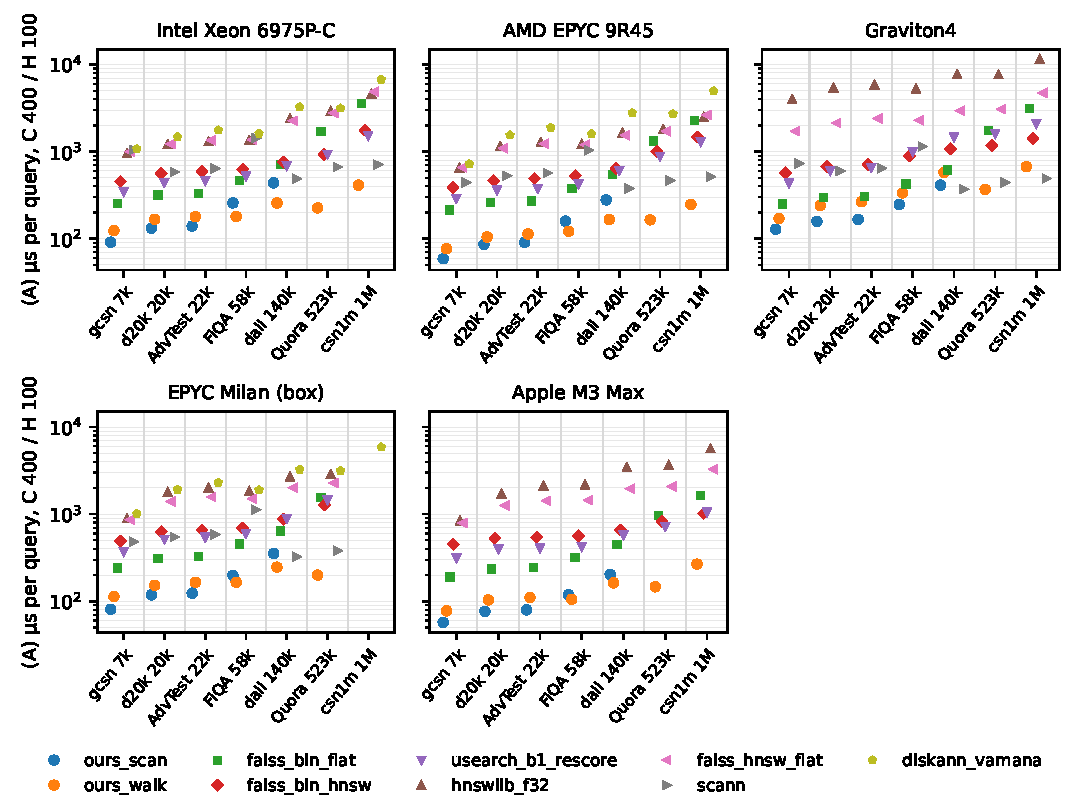
\includegraphics[width=\textwidth]{figures/compA.pdf}
\caption{Comparison (A), held-out, per CPU: \us{} per query of each plotted generator plus the shared
int8 screen and rescoring, at $C = 400$, $H = 100$, smaller declared effort, against corpus size,
with CodeRankEmbed (code sets) and bge-base-en-v1.5 (BEIR sets). FAISS RaBitQ flat and IVF are in the
tables only. Retained quality per cell is in Tables~\ref{tab:compA-intel}--\ref{tab:compA-mac}.}\label{fig:compA}
\end{figure}

\compAtable{intel}{Intel Xeon 6975P-C}

\subsection{Comparison (B): as shipped, at the same retained quality}

Table~\ref{tab:headline099} compares our cascade with the rival that was fastest \emph{on dev} at
$\fr = 0.99$, each at its frozen point; held-out data decide nothing about which rival is shown. The
table marks where our point ($\dagger$) or the rival's ($\ddagger$) misses $\fr$ on held-out by its point
estimate. Figure~\ref{fig:size} plots our cascade against corpus size. On these sets, the ratio
depends on corpus size more than on the CPU.

\begin{itemize}\setlength{\itemsep}{1pt}
\item \textbf{Large sets} (Quora, 523k vectors; csn1m, 1M): ours is faster in \nm{faster-large} of
\nm{n-large} cells (whole interval above 1) and slower in \nm{slower-large}; ratios \nm{min-large} to
\nm{max-large}, geometric mean \nm{gm-large}. The rivals here are graph indexes: FAISS HNSW (float32,
SQ8, binary or RaBitQ codes), USearch b1, and SVS Vamana with LVQ or LeanVec on Intel. Several large-set
intervals are wide because of slow rounds of our cascade (\S\ref{sec:losses}).
\item \textbf{Middle sets} (FiQA, 58k; dall, 140k): mixed. Ours is faster in \nm{faster-mid} of
\nm{n-mid} cells and slower in \nm{slower-mid} (geometric mean \nm{gm-mid}).
\item \textbf{Small code sets} (gcsn, d20k, AdvTest; 7k--22k): the rivals are faster in most cells. Ours
is slower in \nm{slower-small} of \nm{n-small} cells and faster in \nm{faster-small} (geometric mean
\nm{gm-small}). The rival is usually FAISS binary flat: an exact Hamming scan of the same 512-bit codes,
followed by float refine, in C++.
\end{itemize}

Over all CPUs and sets, the geometric mean of the ratio at $\fr = 0.99$ is \nm{gm-all-099}
(\nm{gmn-all-099} cells, ours faster by point estimate in \nm{wins-all-099}); per CPU it is
\nm{gm-intel-099} (Intel), \nm{gm-amd-099} (AMD), \nm{gm-arm-099} (Graviton), \nm{gm-box-099} (box,
reduced grid) and \nm{gm-mac-099} (Mac, reduced grid). At $\fr = 0.995$ it is \nm{gm-all-0995}
(Appendix~\ref{app:fractions}). The four code sets gcsn, d20k, dall and csn1m share one query set, so
their cells are four sizes of one test, not four independent tests; the geometric means are descriptive.
The large sets are mostly faster and the small code sets mostly slower on every CPU, while some middle
cells change sign between CPUs (FiQA with bge: 0.88 on Intel, 0.69 on AMD, 1.41 on Graviton).

\headlinetable{0.99}{099}

\begin{figure}[t]\centering
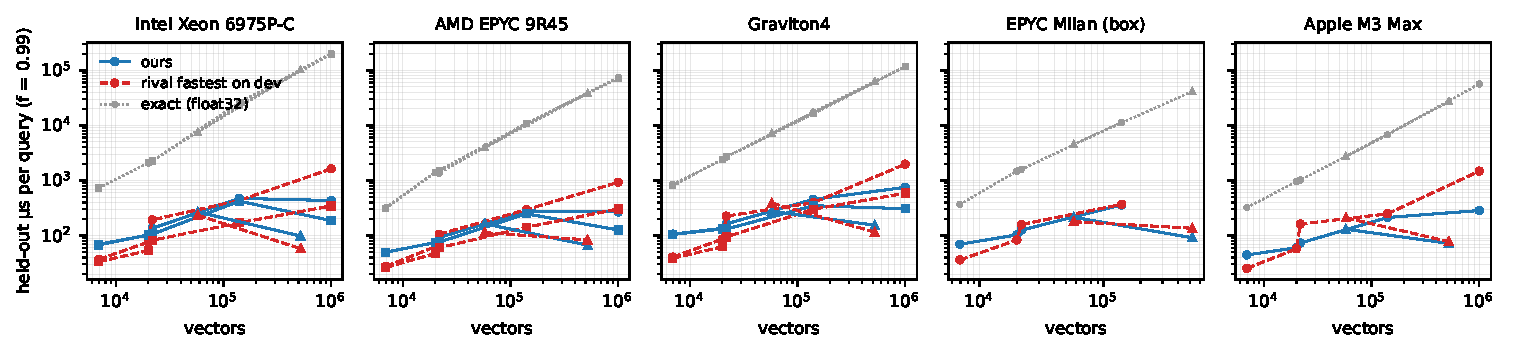
\includegraphics[width=\textwidth]{figures/size.pdf}
\caption{Comparison (B), held-out, $\fr = 0.99$, per CPU: our cascade (blue), the rival that was fastest on dev
at $\fr$ (red, dashed; Table~\ref{tab:headline099}) and exact float32 search (grey), against corpus size. Circles and squares: code sets with CodeRankEmbed and
jina; triangles: BEIR sets with bge-base-en-v1.5.}\label{fig:size}
\end{figure}

\paragraph{Held-out re-test of the dev points.} Every frozen point met its fraction on dev with the
one-sided 97.5\% bound. On held-out queries at $\fr = 0.99$, all \nm{ret-ours-n} of our points meet it by
the point estimate and \nm{ret-ours-bound} (\nm{ret-ours-boundpct}\%) by the bound; of the
\nm{ret-riv-n} rival points, \nm{ret-riv-point} (\nm{ret-riv-pointpct}\%) meet it by the point estimate
and \nm{ret-riv-bound} (\nm{ret-riv-boundpct}\%) by the bound. A point chosen as the fastest that passes
on dev sits close to the boundary, so a fresh sample moves it either way; we report the re-test and do
not re-select.

\paragraph{Tuning budget.} The dev selection gave each system its own declared grid
(Table~\ref{tab:tuning}): up to \nm{tune-max} configurations per set and model for the graph families
with refine, and \nm{tune-ours} for our cascade. Our production defaults were tuned earlier on the gcsn
dev queries, outside this study.

\begin{table}[t]\centering\scriptsize
\caption{Tuning budget: distinct comparison-(B) configurations per set and model in the dev sweep
(including the widened IVF and ScaNN grids), per AWS CPU. Empty: the system does not run on that CPU.}\label{tab:tuning}
\begin{tabular}{lrrr}\toprule
System & Intel & AMD & Graviton\\\midrule
\inputtable{tables/tuning.tex}
\bottomrule\end{tabular}
\end{table}

\paragraph{Hamming ties (dev only).} Sign codes produce many equal Hamming distances. On gcsn dev with
CodeRankEmbed, the run of tied candidates crosses the stage-1 cut at $C = 400$ on 97.8\% of queries;
changing the order inside tie runs changes the retained candidate set on about 28\% of queries, the
top-10 documents on about 1.6\%, and MRR@10 by at most 0.0001 over five random tie orders. This analysis
ran on dev before the freeze, with vectors from an earlier embedding run of the same model.

\subsection{Primary comparisons}

Table~\ref{tab:primary} gives the \nm{nprimary} primary pairs. Following the plan, a pair whose power
on dev was below 0.8 is reported descriptively: \nm{ndescr} pairs (FiQA with bge-base-en-v1.5 on AMD and
Graviton). Quality non-inferiority at $\delta = \nm{delta}$ passes in \nm{nprimarypass} of the
\nm{nconfirm} confirmatory pairs after Holm; the failure is FiQA with bge-base-en-v1.5 on Intel
(observed difference $-0.0015$, 259 held-out queries). On latency, which is descriptive, ours is faster in
\nm{nprimaryfaster} pairs and slower in \nm{nprimaryslower} (whole interval on one side of 1). Two of the
slower pairs compare against a rival point that misses $\fr$ on held-out (FiQA with jina: SVS LVQ on
Intel and hnswlib on AMD), so they are not at matched quality.

\begin{table}[t]\centering\scriptsize
\caption{Primary pairs (fixed on dev; $\fr = 0.99$, comparison B). Ratio: rival / our latency (median over
rounds, 95\% bootstrap interval over rounds). Meets: point estimate / bound, for ours ; rival. Quality:
mean of per-query nDCG@10 (ours $-$ rival) and its one-sided 97.5\% lower bound; non-inferiority at
$\delta = \nm{delta}$, Holm over the \nm{nconfirm} confirmatory pairs; descr.: power below 0.8 on dev,
descriptive.}\label{tab:primary}
\setlength{\tabcolsep}{3pt}
\begin{tabular}{llllrlrrrl}\toprule
CPU & Set & Model & Rival & Ratio & Meets & Mean diff & Lower & $p$ & Holm\\\midrule
\inputtable{tables/primary.tex}
\bottomrule\end{tabular}
\end{table}

\subsection{Memory, load and build}

Table~\ref{tab:mem-csn1m} shows memory and cold start at 1M vectors on the Linux machines (Quora and dall
in Appendix~\ref{app:mem}). Our cascade holds the graph, the codes, the int8 rows and the float16
vectors, memory-mapped from its index files, plus the Node.js runtime: \nm{mem-ours-intel}~GiB on Intel
(\nm{mem-ours-amd} on AMD, \nm{mem-ours-arm} on Graviton), more than \nm{mem-smaller-intel} of the
\nm{mem-nriv-intel} rival points on Intel. The smallest is USearch int8 at \nm{mem-rivalmin-intel}~GiB;
the rivals that refine with float32 originals use 3.0--3.6~GiB, and FAISS HNSW-SQ8
\nm{mem-rivalmax-intel}~GiB. Our cold start (load plus first query after the page cache is dropped) is
\nm{cold-ours-intel}~s on Intel against \nm{cold-rivalmin-intel}--\nm{cold-rivalmax-intel}~s for the
rivals; the rival numbers include the harness's buffered read of the originals (\S\ref{sec:systems}), so
this comparison is indicative. Table~\ref{tab:build} lists build cost at 1M: our build took
\nm{build-ours-s}~s (\nm{build-ours-h}~hours) of wall time on one thread with a peak of
\nm{build-ours-peak}~GB, the longest wall time of any build (the longest rival build took
\nm{build-rival-max-s}~s on 16 threads). In core-seconds our build is below the largest rival graph
builds.

\memtable{csn1m}{csn1m, CodeRankEmbed}

\begin{table}[t]\centering\scriptsize
\caption{Build cost at 1M vectors (csn1m, CodeRankEmbed), one row per family: the range over its
build grid. Builds ran under a memory-admission scheduler, several at a time, so wall times are
indicative. Core-seconds = wall time $\times$ threads (an upper bound for the concurrent rival builds).}\label{tab:build}
\begin{tabular}{lrrrrrr}\toprule
Family & Builds & Wall s & Threads & Core-s & Size GB & Peak RSS GB\\\midrule
\inputtable{tables/build.tex}
\bottomrule\end{tabular}
\end{table}

\section{Post-freeze experiments}\label{sec:post}

The experiments in this section ran after the held-out run, on held-out queries, with the frozen builds
and operating points and with harness changes that only add clocks and switches (Appendix~\ref{app:deviations}).
They answer two questions that the main results leave open; they are not part of the pre-registered study.

\subsection{Generator time alone}

We added per-query clocks around the stages of comparison (A) in both harnesses: query conversion, the
generator, and the shared screen plus rescoring. We reran (A) at $C = 400$, $H = 100$ on the three AWS CPUs
(one model per set kind, 5 rounds), with every declared effort, with the four graph families also at the
build our graph uses ($M = 64$, $ef_{\text{construction}} = 800$), and with our walk also at a fixed $ef$,
without early termination and without huge pages.

\paragraph{Shared stages.} The screen plus rescoring took a median \nm{post-shared-ours-intel}~\us{} in our
implementation and \nm{post-shared-riv-intel}~\us{} in the rivals' C++ path on Intel
(\nm{post-shared-x-intel}$\times$), \nm{post-shared-x-amd}$\times$ on AMD and \nm{post-shared-x-arm}$\times$ on
Graviton: the gap estimated in \S\ref{sec:results} is real and of that size.

\paragraph{Generators at equal settings.} With the same graph build ($M = 64$), the same $ef$, our walk
without its adaptive rule, early termination or huge pages, and the generator clock alone, the rival
graph generators took \nm{post-eq-min} to \nm{post-eq-max} times as long as our walk (geometric mean
\nm{post-eq-gm}, \nm{post-eq-n} comparisons; ours faster in \nm{post-eq-ours}). Table~\ref{tab:postgen}
gives, per CPU and set, the generator time of the fastest of our configurations and of the fastest rival
configuration among those whose retained quality is at least 99\%; by generator time alone, ours is the
fastest in \nm{post-best-ours} of \nm{post-cells} cells.

\begin{table}[h]\centering\scriptsize
\caption{Post-freeze (A), held-out, $C = 400$, $H = 100$: generator time alone (median over rounds of the
per-round median, \us{}) of the fastest of our configurations and of the fastest rival configuration with
retained quality $\ge 0.99$, and their ratio.}\label{tab:postgen}
\begin{tabular}{llrlrr}\toprule
CPU & Set & Ours \us{} & Rival & Rival \us{} & Ratio\\\midrule
\inputtable{tables/post-gen.tex}
\bottomrule\end{tabular}
\end{table}

\subsection{Slow rounds and the large sets in comparison (B)}

Every record of the post-freeze runs counts the major page faults of its timed pass. Our cascade had
\nm{post-slow-ours} slow rounds in \nm{post-rounds-ours}, the rivals \nm{post-slow-riv} in
\nm{post-rounds-riv}. Every slow round of ours had at least \nm{post-slow-faults-min} major page faults in its timed pass
(median \nm{post-slow-faults-med}), against a median of \nm{post-fast-faults-med} in our other rounds. So
in a slow round, pages of our memory-mapped files were read from disk during the timed pass, although
the pre-read before the job had loaded them: they had been evicted in between. In comparison (A) the stage
clocks place the extra time of 12 of the 16 slow rounds in the full-vector rescoring (the float16 vector
file) and of the other 4 in the int8 screen (the int8 rows); the generator is never the slow stage. A
server whose index shares the page cache with other I/O can see the same effect; the rivals, which read
their indexes into anonymous memory, cannot.

On Quora and csn1m we reran our frozen point and the rival fastest on dev at $\fr = 0.99$, with the CPU's
$R$ rounds (Table~\ref{tab:postb}). The geometric mean of the ratio over the \nm{postb-n} cells is
\nm{postb-gm} (ours faster by point estimate in \nm{postb-wins}). The native calls of our cascade take
\nm{postb-native-min}--\nm{postb-native-max}\% of its timed query (median \nm{postb-native-med}\%); the rest
is JavaScript orchestration and metadata reads. Our shipped default ($S_1 = 400$) takes
\nm{postb-default-tmin}--\nm{postb-default-tmax} times the time of our frozen point: more where the frozen point
uses a smaller $S_1$ (below the product floor), less on csn1m with bge, where the frozen point uses
$S_1 = 2000$ or 3000 and the default retains only \nm{postb-default-qmin} of exact quality, below
$\fr = 0.99$.

\begin{table}[h]\centering\scriptsize
\caption{Post-freeze (B), held-out, $\fr = 0.99$, Quora and csn1m: rival / our latency of the rerun
(median over rounds, 95\% bootstrap interval), our slow rounds, the native share of our time, and our
shipped default ($S_1 = 400$) as time relative to our frozen point / retained quality.}\label{tab:postb}
\begin{tabular}{llllrrrl}\toprule
CPU & Set & Model & Rival & Ratio & Slow & Native & Default\\\midrule
\inputtable{tables/post-b.tex}
\bottomrule\end{tabular}
\end{table}

\section{Pre-registered replication on untouched sets}\label{sec:replication}

The main results are descriptive (\S\ref{sec:limits}, Appendix~\ref{app:deviations}). To test the speed claim
once, we ran a replication on two sets that no earlier step used, with a corrected harness and rules written and
committed before any replication data existed (\texttt{REPLICATION\_PLAN.md}); two independent pre-run reviews of
the harness and the plan were applied before the first timing run.

\paragraph{Design.} CQADupStack (all 12 forums merged; 457,199 documents; 13,145 queries, split by forum) and an MS
MARCO subsample of 1,000,000 passages (every passage judged for a dev query plus a seeded random sample; 6,980
queries), embedded with bge-base-en-v1.5. One build per rival family (the build most often frozen for that family in
the main study), every effort-type knob on the same 11-value grid as our stage-1 size, and our cascade only at
configurations the product itself runs. Dev selection at $\fr = 0.99$ used the median of three timed rounds; the rival
of each test is the rival fastest on dev. Rival timers compute only the query forms the family uses, each job
pre-reads only the files it opens, and a job with more than 1,000 major page faults in its timed pass runs once more
(invalid if it fails again). On held-out queries, each CPU type ran 6 fresh instances, each with 2 blocks that hold
ours and every frozen rival point in a seeded random order. The latency test is a one-sided $t$-test over the 6
instance means of log(rival / ours); the quality test is non-inferiority with a relative margin of 0.5\% of exact
quality, bootstrapped jointly over queries; each family of 6 tests is Holm-corrected at 0.025; a set--CPU pair counts
as ``faster at 99\% quality'' only if both tests pass.

\paragraph{Results.} Table~\ref{tab:rep} gives the six pairs. The latency test passes in \nm{rep-lat-pass} of
\nm{rep-n}, the quality test in \nm{rep-q-pass} of \nm{rep-n}, and both in \nm{rep-joint} of \nm{rep-n}. The
geometric mean ratio over instances is \nm{rep-gm} (from \nm{rep-min} to \nm{rep-max}). \nm{rep-reruns} jobs were
rerun by the fault rule and \nm{rep-dropped} blocks were dropped. At the 99th percentile the ratio is \nm{rep-p99};
the native calls are \nm{rep-native}\% of our timed query.

The quality test separates the two sets. On MS MARCO 1M it passes on all three CPUs, so the joint claim (faster and
not worse than the dev-chosen rival by more than 0.5\% of exact quality) holds there on every CPU. On CQADupStack it
fails on all three CPUs: the mean difference to the rival is between $-0.0010$ and $0.0000$ nDCG@10, but its lower
bound falls just below the margin of 0.0021, and both our point and the rival's meet $\fr = 0.99$ only by the point
estimate, not by the bound. The latency advantage on CQADupStack is therefore shown, but quality non-inferiority at
this margin is not; we do not claim it.

\begin{table}[h]\centering\scriptsize
\caption{Replication, held-out, $\fr = 0.99$ (pre-registered tests). Ratio: geometric mean over the 6 instances of
rival / ours (paired bootstrap interval over instances). Latency: one-sided $t$-test, Holm over 6. Quality: mean of
per-query nDCG@10 (ours $-$ rival) and the non-inferiority test at 0.5\% of exact quality, Holm over 6.}\label{tab:rep}
\setlength{\tabcolsep}{3pt}
\begin{tabular}{lllrrrrrlrrl}\toprule
CPU & Set & Rival & Inst. & Ours \us{} & Rival \us{} & Ratio & $p$ (lat.) & Holm & Mean diff & $p$ (qual.) & Holm\\\midrule
\inputtable{tables/rep.tex}
\bottomrule\end{tabular}
\end{table}

\section{Post hoc checks on the replication sets}\label{sec:posthoc}

After the replication we ran four checks on the replication sets, held-out, with the replication's builds, frozen
points, fault rule and instance types. They were planned and frozen with file hashes before they ran
(\texttt{POSTHOCFREEZE.json}), but they come after the replication results and are descriptive.

\paragraph{The six tests with the index preloaded.} The replication's one weak point was the page cache: every fault
rerun was a job of ours, and one pass depended on dropping a faulted block (\S\ref{sec:replication}). We added a product
option that reads the int8 rows and the float16 vectors into anonymous memory at load instead of mapping them
(\texttt{SS\_HNSW\_PRELOAD=1}; result lists byte-identical to the mapped index) and ran the six tests again with the same
plans, seeds and 6 fresh instances per CPU type, every job of ours preloaded. All \nm{pl-n} latency tests pass
(Table~\ref{tab:preload}; ratios \nm{pl-min}--\nm{pl-max}, geometric mean \nm{pl-gm}), with all \nm{pl-blocks} blocks kept,
\nm{pl-reruns} fault reruns and \nm{pl-dropped} dropped blocks. Preloading made our query \nm{pl-slow}\% slower (geometric mean) and
gives up the lazy loading of \S\ref{sec:results}, but the speed result no longer depends on the fault rule. The option stays off by default:
it reads about 2~GB at 1M vectors (int8 rows 0.5~GB, float16 vectors 1.5~GB) before the first query, where the
mapped index loads lazily, and it keeps that memory
anonymous and unreclaimable, where the mapping lets the operating system reclaim pages under memory pressure. The quality
tests read the same lists and give the same results (\nm{pl-qpass} of \nm{pl-n}).

\begin{table}[h]\centering\scriptsize
\caption{Post hoc: the six replication latency tests with our index preloaded into anonymous memory, held-out, same plans
and test as Table~\ref{tab:rep}. Before: the pre-registered ratio of Table~\ref{tab:rep}. Faults: jobs rerun by the fault
rule.}\label{tab:preload}
\setlength{\tabcolsep}{3pt}
\begin{tabular}{lllrrrrrrlr}\toprule
CPU & Set & Rival & Before & Blocks & Ours \us{} & Rival \us{} & Ratio & $p$ & Holm & Faults\\\midrule
\inputtable{tables/rep-preload.tex}
\bottomrule\end{tabular}
\end{table}

\paragraph{Comparison (A) with common kernels and a true int8 bypass.} We ported our SIMD kernels to the rivals' shared C++
path (int8 dot products, float16 widening and 16-row float64 dot products; the retained lists are byte-identical to the
scalar path), added a switch that skips the int8 stage entirely in both harnesses (no int8 reads and no sort; every
candidate goes to the float16 rescoring in generator order), and ran comparison (A) at $C = 400$ on both replication
sets: our walk (preloaded, production adaptive rule) against the rival graphs at their replication builds and FAISS
binary flat with its counting top-$k$, every graph at effort 400 (one instance per CPU type, 5 rounds;
Table~\ref{tab:strong}). The shared stages now cost the rivals \nm{st-shared-min}--\nm{st-shared-max} times what they cost
ours, so the earlier kernel gap is gone; the fastest rival generator that keeps 99\% of exact quality still takes
\nm{st-next-min}--\nm{st-next-max} times as long as ours in total. The int8 screen saves time: without it, rescoring all 400 candidates was slower in \nm{byp-slower} of
\nm{byp-n} system--set--CPU cases (ours \nm{byp-ours-min}--\nm{byp-ours-max}~\us{} slower), with the same retained quality.

\begin{table}[h]\centering\scriptsize
\caption{Post hoc comparison (A), held-out, $C = 400$, common SIMD kernels in the shared stages: \us{} per query (median over
5 rounds; in brackets generator + shared stages) with the int8 screen ($H = 100$) and with no int8 stage ($H = 400$,
``bypass''), for our walk and for the fastest rival generator that keeps 99\% of exact quality; Ratio: rival / ours with
the screen; retained share of exact nDCG@10, ours ; rival.}\label{tab:strong}
\setlength{\tabcolsep}{3pt}
\resizebox{\textwidth}{!}{\begin{tabular}{llrrlrrrl}\toprule
CPU & Set & Ours & Ours, bypass & Rival & Rival & Rival, bypass & Ratio & Retained\\\midrule
\inputtable{tables/strong-a.tex}
\bottomrule\end{tabular}}
\end{table}

\paragraph{Float16 refine for the rivals.} The refining dev-chosen rivals (FAISS HNSW-SQ8 on AMD, FAISS binary HNSW on
Graviton) ran their frozen points with the float16 rows instead of the float32 originals in the refine step
(\nm{f16-n} cases). Their time changed by a factor of \nm{f16-tmin}--\nm{f16-tmax} and their retained share by at most
\nm{f16-qmax}: in these three cases the refine representation does not explain the comparison (B) results.

\paragraph{Where FAISS binary HNSW spends its time.} On MS MARCO dev, with the same codes, $M = 64$ builds and a fixed
$ef = 400$ (our walk without its adaptive rule), \texttt{perf stat} counted each process over the full dev split and over
one query; the difference per query is in Table~\ref{tab:perf}. Our walk computes slightly more Hamming distances than
FAISS (\nm{perf-ndis-ours} against \nm{perf-ndis-faiss} per query), so it does not win by skipping work. FAISS executes
\nm{perf-ins-x-intel}--\nm{perf-ins-x-amd} times as many instructions, has \nm{perf-br-x-intel}--\nm{perf-br-x-arm} times as many branch
misses and takes \nm{perf-cyc-x-intel}--\nm{perf-cyc-x-amd} times as many cycles; about 190 instructions per distance against
50--75 for ours (ours includes its JavaScript call). \texttt{perf record} puts 35--52\% of FAISS's time in its per-candidate
Hamming distance call, 17--23\% in the search loop and about 13--16\% in its heaps. Our walk filters visited nodes without
branches, scores a whole neighbour list in one batch and keeps bucket queues (\S\ref{sec:post}); the counters are consistent with these choices, not with fewer distances, as the source
of the gap; they do not measure the share of each choice. A FAISS setting we did not find could close part of it; the counting top-$k$ of the flat
index (\S\ref{sec:post}) shows that defaults matter, and we will report any correction.

\begin{table}[h]\centering\scriptsize
\caption{Post hoc \texttt{perf stat} per query, MS MARCO 1M dev, same codes, $M = 64$, fixed $ef = 400$: Hamming distances
computed, cycles and instructions (millions), branch misses (thousands), and instructions per distance. Ours includes its
JavaScript call and its shared stages; FAISS ran with the ported SIMD shared path, so its counts are not inflated
by the scalar rescoring.}\label{tab:perf}
\begin{tabular}{llrrrrr}\toprule
CPU & Walk & Distances & Cycles (M) & Instr. (M) & Br. misses (k) & Instr./distance\\\midrule
\inputtable{tables/perf.tex}
\bottomrule\end{tabular}
\end{table}

\section{Where the cascade loses}\label{sec:losses}

We list the losses in the main text because they bound what the results support.

\paragraph{Small corpora.} On the small code sets (7k--22k vectors) the rivals win more often than we
do: ours is slower in \nm{slower-small} of \nm{n-small} cells at $\fr = 0.99$, down to a ratio of
\nm{min-small} (the rival takes \nm{min-small} of our time). The winner is usually FAISS binary flat,
which does the same first step as our cascade on these sets (an exact Hamming scan of 512-bit codes)
and then refines in float. At this size the scan is cheap, so the fixed per-query cost of the rest of
the pipeline decides; our cascade adds an int8 stage and runs its orchestration in Node.js. We did not
profile this cost, so we do not attribute the gap to one stage.

\paragraph{Specific rivals at scale.} On Quora with bge-base-en-v1.5, SVS Vamana with LeanVec on Intel
and FAISS binary HNSW on Graviton are faster than ours at $\fr = 0.99$, and both are primary
comparisons. SVS (LVQ or LeanVec) also beats us on FiQA on Intel. SVS runs on Intel only in this
study, so we cannot say how it would fare on the other CPUs.

\paragraph{Quality on FiQA.} On FiQA with CodeRankEmbed our cascade never reached 99\% of exact quality
on dev, so it has no operating point there at that fraction. On FiQA with bge-base-en-v1.5 the
non-inferiority test fails on all three CPUs: the held-out set has 259 queries and the power of these
comparisons was the lowest of all (Appendix~\ref{app:power}). The data do not show a loss larger than
$\delta$, but they do not exclude one.

\paragraph{Memory and build.} At 1M vectors our process holds more memory than \nm{mem-smaller-intel}
of the \nm{mem-nriv-intel} rival points on Intel. It keeps the graph with the codes and int8 rows
(1.2~GB of index file at 1M) and the float16 vectors (1.5~GB), plus the Node.js runtime; rivals that
refine keep float32 originals but a smaller graph, and quantised graphs without refine keep far less. Our index build is single-threaded and took \nm{build-ours-h}~hours
with a \nm{build-ours-peak}~GB peak at 1M; every rival build finished faster on 16 threads. A parallel
build is possible but was out of scope for this study.

\paragraph{Sensitivity to page-cache pressure.} Our index is memory-mapped. In \nm{outlier-ours} of
\nm{records-ours} held-out records of our cascade (\nm{outlier-share}), all on Quora and csn1m, the
per-round median query time was more than three times that of the fastest round of the same point, up
to several hundred times. No record of the \nm{records-rival} rival records had such a round; the rivals
read their indexes into anonymous memory. The slow rounds cluster on a few machine instances. We did not
establish the cause; eviction of file pages by other I/O on the machine (for example the periodic
upload of large result files) is the most likely one. Our reported latency is the median
over rounds, which such a round does not move, and our ratio intervals come from a bootstrap of
medians; but the intervals of the affected cells are wide (Table~\ref{tab:headline099}), and a server
that shares its page cache with heavy I/O can see the same effect. Locking the index in memory, or
reading it into anonymous memory, would remove it at the cost of a longer load.

\section{Limits}\label{sec:limits}

\paragraph{Sizes and dimensions.} The sets hold 7k to 1M vectors. We make no claim beyond 1M vectors,
where memory-resident flat scans stop being an option and graph and partition indexes have more room
to pay off. All vectors have 768 dimensions; our codes use the first 512. Other dimensions, and models
whose leading dimensions carry less of the signal, can change the result.

\paragraph{Models and tasks.} Three embedding models, five code-search sets and two BEIR sets. The
code-search results are exploratory: the code queries were examined in earlier work on the same
system, and dev and held-out code queries share most source repositories (the bootstrap resamples
repositories, which accounts for this inside a set but not across sets). The confirmatory part is
the \nm{nprimary} primary comparisons on Quora and FiQA.

\paragraph{Machines.} Every Linux machine is a virtual machine, so page sizes, frequency and
neighbour load are not under our control. A/A runs measured this noise per machine and set $R$; the
rounds of one point usually ran on different instances, so instance-to-instance variation is inside
the intervals. Results on bare metal can differ, in particular for the graph walks, whose cost depends
on TLB behaviour. The Mac runs unpinned. The box and the Mac run a reduced grid.

\paragraph{Single queries, single thread.} We time one query at a time on one core. Batched search,
multi-threaded search and shared-index throughput are out of scope; several rivals (FAISS flat
scans, IVF) gain more from batching than graph walks do. Our index build is single-threaded; the
rival builds used the thread counts in Table~\ref{tab:build}. Build cost is indicative only
(\S\ref{sec:systems}).

\paragraph{Tested interfaces.} Each rival is used through the interface we wrapped: the C++ API for
FAISS, hnswlib, USearch, DiskANN and SVS, and the Python binding for ScaNN. Another interface,
another build of the same library, or parameters outside the declared grids can be faster. We
declared the grids before the dev runs and widened two (IVF probes and ScaNN leaves) on dev, before
the freeze, when those families did not reach the fractions.

\paragraph{Our harness.} Our system runs in Node.js with a native addon, the rivals in C++ (ScaNN in
Python). Comparison (A) runs our generators through the addon and the shared steps in both C++ and the
addon with bit-identical lists, so the generator times include the language boundary of each system.

\paragraph{The reporting script.} \texttt{analyze.py} was written after the freeze. It applies the
frozen rules with the frozen quality and statistics code and selects nothing; we release it with the
data so that every table can be checked against the raw records.

\section{Reproducibility}\label{sec:repro}

The harness, the adapters, the plans, the frozen operating points and \texttt{FREEZE.json} are in
the repository~\cite{sweetsearch_repo} under \texttt{eval/benchmarks/hnsw-rivals/paper} (frozen
commit \texttt{f57533b0}, tag \texttt{hnsw-rivals-freeze-2026-10-17-v2}). The release adds the
vectors of every set and model, the splits, the ground truth, every held-out result record with its
retained lists, and the per-job timing files. From these, one command rebuilds each table and
figure:

\begin{small}\begin{verbatim}
python analyze.py --data DATA --results RESULTS --shortlists shortlists \
    --builds BUILDS --types T --out R-T.md --json J-T.json  # per CPU T
python merge_results.py --parts . --out RESULTS-paper.md \
    --json results-paper.json
python mem_patch.py --results RESULTS --json results-paper.json
python draft/mktex.py results-paper.json --extra draft/extra.json
python draft/figures.py results-paper.json
\end{verbatim}\end{small}

\texttt{freeze\_check.py} confirms that the frozen files are unchanged, and
\texttt{check\_complete.py} confirms that every planned held-out job has a complete record
(\nm{hojobs} jobs on the three AWS CPUs). Adding a system takes one adapter with the common
interface (build, load, search, return a vector list with scores) and its build and search grids in
\texttt{grid.py}; the selection and analysis scripts need no change. \TODO{release kit: a small laptop example (gcsn, one model, two systems), its measured run time, and the archive DOI}

\section{Conclusion}\label{sec:conclusion}

Measured at a fixed fraction of task quality instead of a recall target, and with the rest of the
pipeline held fixed, the binary scan and binary HNSW walk were the fastest candidate generators
wherever they kept 99\% of exact quality, on five CPUs; part of that margin is our faster implementation of
the shared steps, but per-stage clocks at equal graph settings confirm it for the generator alone; float32 graphs kept that quality at smaller
candidate budgets for some model--set pairs. As shipped, the binary cascade was faster than the rival
chosen on dev in most cells at 0.5M--1M vectors and slower than an exact binary scan in C++ on most code
sets below about 20k vectors. Its costs are memory, a slow single-threaded build, a longer latency tail, and
page-cache misses of its memory-mapped files under other I/O. These results hold for the tested sets, models and CPUs, within the declared quality margin; the released
records let others check them and add systems.

\section*{Use of AI assistants}

AI coding assistants were used throughout this work. Claude (Anthropic), through Claude Code, wrote most of the
benchmark harness, adapters and analysis scripts, operated the cloud runs within budgets and approvals set by the
author, and drafted much of this text. Claude models and OpenAI Codex models reviewed the protocols and drafts. The author
chose the research question, approved the protocol, the freezes and every paid run, and is responsible for the content.
Every number in the text is generated from the released records by the released scripts.


\bibliographystyle{plainurl}
\bibliography{refs}

\appendix
\section{Deviations from the plan}\label{app:deviations}

Table~\ref{tab:deviations} lists every departure from the pre-registered plan that we know of, with
when it happened relative to the freeze and to the held-out run, and where its effect is reported.

\begin{table}[h]\centering\scriptsize
\caption{Deviations from the pre-registered plan. ``Before freeze'' changes used dev data only.}\label{tab:deviations}
\begin{tabularx}{\textwidth}{p{3.6cm}p{2.1cm}X}\toprule
Deviation & When & Effect and where reported\\\midrule
Our (B) grid widened ($S_1$ = 1500, 2000, 3000), because csn1m with bge reached 99\% only at the grid's
top & before freeze, after the first dev sweep & frozen points at these values: csn1m--bge at $\fr = 0.99$ on all AWS CPUs, dall--bge at 0.995, one FiQA point; rival effort grids were not widened (IVF probes and ScaNN leaves were, for coverage) \\
Warm page cache added before each job; only our (B) and all (A) dev jobs rerun & before freeze & rival (B) dev selection uses the first sweep; held-out uses the warm protocol for every system \\
Our (B) runs below the product's stage-1 floor (a bench-only override) and ties $ef$ to $S_1$ & declared before freeze & \nm{ours-below-floor} of our \nm{ret-ours-n} frozen points at $\fr = 0.99$ are configurations the product does not run (\S\ref{sec:systems}) \\
Freeze record rewritten after a run-script change & before any held-out job & file hashes unchanged (commit 4a0d8842); record at f57533b0 \\
Box and Mac: points borrowed from the AMD and Graviton shortlists; $R$ from their own A/A runs (10 and 4) & after freeze & secondary rows; not comparable with the AWS geometric means (\S\ref{sec:limits}) \\
Box csn1m: only DiskANN ran (disk full) & held-out run & box csn1m left out of all tables \\
\nm{repairjobs} held-out jobs re-run after a machine time limit (AMD FiQA--jina, AMD Quora--jina, Intel dall--bge, Intel dall--jina, Graviton dall--jina, Graviton FiQA--CRE) & held-out run, same frozen code & complete records for every planned job \\
Reporting code written after the freeze: \texttt{analyze.py}, \texttt{merge\_results.py}, \texttt{paperlib.py}, \texttt{mem\_patch.py}, \texttt{mktex.py}, \texttt{figures.py} & after the held-out run & see the next three rows \\
Ratio statistic: median over rounds with a bootstrap interval; the first reporting script used the mean of log round medians (Welch $t$) & changed after the held-out results were seen (slow rounds of ours) & both reported (\S\ref{sec:results}, sensitivity) \\
Headline rival: first chosen as the fastest rival meeting $\fr$ on held-out; now the rival fastest on dev & changed after the held-out results & dev rule is the plan's; held-out rule not reported \\
Memory on Linux read from the right field; Mac memory not reported & after the held-out results & \S\ref{sec:systems} \\
Primary pairs with dev power below 0.8 made descriptive (the plan's rule) & after the held-out results (the rule was not applied at first) & \nm{ndescr} pairs descriptive \\
Comparison (A): the shared screen and rescoring are bit-identical in output but run in our SIMD kernels for ours and in a scalar C++ path for the rivals; rival graphs $M = 32$, ours $M = 64$ & design, before freeze & (A) ratios with the rescoring difference removed by estimate (\S\ref{sec:results}) \\
Comparison (B): rival refine is one harness routine, not each library's own; the rival timer includes an unneeded query conversion & design, before freeze & \S\ref{sec:systems}; not measured separately \\
Post-freeze experiments: stage clocks in (A), $M = 64$ rival graphs, our walk with fixed $ef$, page-fault counts, (B) rerun on Quora and csn1m with native-only clocks and the shipped default; harness changes add clocks and switches only (record \texttt{POSTFREEZE.json}) & after the held-out run & \S\ref{sec:post}, reported apart \\
Not run: two build seeds, isolated build-cost runs, first-100 cold queries, page-policy arms, dTLB counters & --- & \S\ref{sec:limits} \\\bottomrule
\end{tabularx}
\end{table}


\section{Power of the primary comparisons}\label{app:power}

\begin{table}[h]\centering\scriptsize
\caption{The \nm{nprimary} primary pairs, fixed on dev before the freeze: our time and the rival's at
$\fr = 0.99$ on dev, held-out cluster count, the cluster-bootstrap standard error of the mean quality
difference scaled to held-out, and the power at a true difference of 0 for $\delta = \nm{delta}$
(analytic and by simulation, 2,000 draws).}\label{tab:power}
\begin{tabular}{lllrrrrrrr}\toprule
CPU & Set & Model & Rival & Ours \us{} & Rival \us{} & Clusters & SE & Power & Power (sim)\\\midrule
\inputtable{tables/power.tex}
\bottomrule\end{tabular}
\end{table}

\section{Comparison (B) at the other fractions}\label{app:fractions}

\headlinetable{0.98}{098}
\headlinetable{0.995}{0995}

\begin{table}[h]\centering\scriptsize
\caption{The rival in each cell of Table~\ref{tab:headline099}: the rival that was fastest on dev at $\fr = 0.99$.}\label{tab:fastestrival}
\setlength{\tabcolsep}{3pt}
\begin{tabular}{ll*{5}{l}}\toprule
Set & Model & \inputtable{tables/headline-cols.tex}\\\midrule
\inputtable{tables/fastest-rival-099.tex}
\bottomrule\end{tabular}
\end{table}

\section{Comparison (A) on every CPU}\label{app:compA}

Tables~\ref{tab:compA-intel}--\ref{tab:compA-mac} give comparison (A) per CPU.
The full grid (every budget and both efforts, every set and model) is in \texttt{RESULTS-paper.md}
in the release.

\compAtable{intel}{Intel Xeon 6975P-C}
\compAtable{amd}{AMD EPYC 9R45}
\compAtable{arm}{Graviton4}
\compAtable{box}{EPYC Milan (box)}
\compAtable{mac}{Apple M3 Max}

\section{Memory and cold start}\label{app:mem}

\memtable{quora}{Quora, bge-base-en-v1.5}
\memtable{dall}{dall, CodeRankEmbed}

\section{Tuning budget and build cost}\label{app:extra}

\begin{table}[h]\centering\scriptsize
\caption{Tuning budget: distinct comparison-(B) configurations per set and model in the dev sweep
(including the widened IVF and ScaNN grids), per AWS CPU. Empty: the system does not run on that CPU.}\label{tab:tuning}
\begin{tabular}{lrrr}\toprule
System & Intel & AMD & Graviton\\\midrule
\inputtable{tables/tuning.tex}
\bottomrule\end{tabular}
\end{table}

\begin{table}[h]\centering\scriptsize
\caption{Build cost at 1M vectors (csn1m, CodeRankEmbed), one row per family: the range over its
build grid. Size is the index file only; the refining rivals also need the float32 originals at serving
time (3.09~GB at 1M), while our 2.77~GB includes our float16 vector file. Builds ran under a memory-admission scheduler, several at a time, so wall times are
indicative. Core-seconds = wall time $\times$ threads (an upper bound for the concurrent rival builds).}\label{tab:build}
\begin{tabular}{lrrrrrr}\toprule
Family & Builds & Wall s & Threads & Core-s & Size GB & Peak RSS GB\\\midrule
\inputtable{tables/build.tex}
\bottomrule\end{tabular}
\end{table}


\end{document}
